\chapter{Implementation}
\label{ch:Implementation}

This chapter describes the implementation of the filter algorithm proposed by \citeauthor{bennett_motion_2014} in \cite{bennett_motion_2014}, based on the fundamentals acquired in the previous chapters. Other than in \cite{bennett_motion_2014}, in which the filter algorithm was tested moving a mechanical model of the leg by hand, we used movement data from a human subject. After outlining the initial situation, i.\,e. describing the GaitWatch system, including orientation algorithms that were already implemented, the theoretical design of the filter is elaborated in detail. Subsequently, the software implementation and experiments are presented, followed by the results and their discussion.

\section{Initial Situation}\label{sec:initial_situation}

\subsection{The GaitWatch System}

As indicated above, to gather and preprocess movement data from the subject, we used a system called GaitWatch \cite{olivares_vicente_gaitwatch_2013}, which was designed to monitor the motion of patients by means of inertial sensors attached to the body. It was developed at the Department of Neurology of the Ludwig-Maximilians University in Munich, Germany, in association with the Department of Signal Theory, Telematics and Communications of the University of Granada, Spain.

\subsubsection{Hardware}

From the hardware perspective, the system is composed of a set of magnetic and inertial sensors wired to a box containing a microcontroller. This microcontroller is in charge of collecting data from the sensors embedded in the box, as well as from  external measurement units, and storing them on a memory card. The separate units are placed on the patient's trunk, arms, thighs, and shanks as shown in Figure \ref{fig:GaitWatch_placement}. The components of the three different kinds of subunits are listed below:

\begin{itemize}

\item \textsc{type a -- thighs and shanks:} 

IMU Analog Combo Board with $5$ Degrees of Freedom \cite{IMU5}, containing an IDG$500$ biaxial gyroscope, from which only $y$-axis is actually used, with a measurement range of $\pm500^{\circ}/$s \cite{IDG500} and a $\pm3$\,g triaxial accelerometer, ADXL$335$ \cite{ADXL335}.

\item \textsc{type b -- arms:}

IDG$500$ biaxial gyroscope with a measurement range of $\pm500^{\circ}/$s \cite{IDG500}.

\item \textsc{type c -- trunk:}

ADXL$345$ triaxial accelerometer with a programmable measurement range of $\pm 2/\pm 4/\pm 8/\pm 16$\,g \cite{ADXL345},
IMU$3000$ triaxial gyroscope with a programmable measurement range of $\pm250/\pm500/\pm1000/$ $\pm3000^{\circ}/$s \cite{IMU3000}, 
Micromag$3$ triaxial magnetometer with a measurement range of $\pm11$\,Gauss \cite{MicroMag3}, AL-XAVRB board containing an AVR ATxmega processor \cite{AVRATxmega}.

\end{itemize}

\begin{figure}
\centering
\begin{tikzpicture}[scale=0.95, auto, thick, node distance=3cm,>=latex']
    \pgftext{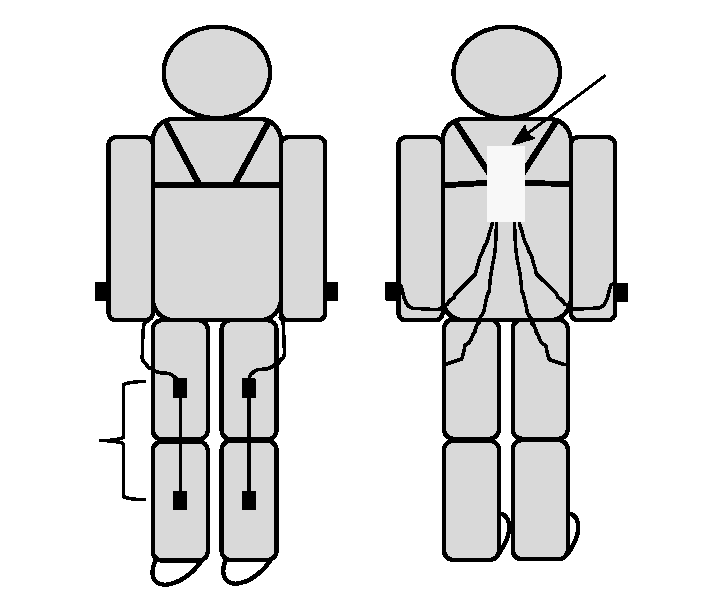
\includegraphics[width=10cm]{Figures/GaitWatch_placement}} at (0pt,0pt);
    \node [] (a) at (-4.4, -2) {Type A};
    \node [] (b) at (-4.5, 0.1) {Type B};
    \node [] (c) at (4.45, 3.25) {Type C};
\end{tikzpicture}
\caption{Placement of the GaitWatch components at the body, from \cite{olivares_vicente_gaitwatch_2013}.}
	\label{fig:GaitWatch_placement}
\end{figure}

\subsubsection{Software}

In addition to the hardware, there was an existing \textsc{Matlab}\textsuperscript{\textregistered} toolbox consisting of routines for reading the data and carrying out the necessary calibration. Also, several algorithms that determine the motion intensity and compute the orientation of the human body from the movement data were already implemented. There were three algorithms for estimating the pitch angle of the thighs and shanks, as described below:

\begin{itemize}
  \item \textsc{projection of the gravity vector:} One way to obtain the pitch angle from the inertial data is using the projection of the gravity vector on the axes of the accelerometer, as described in Section \ref{sec:projection_gravity}. The first algorithm computed the pitch angle according to Equation \ref{eq:projection_gravity}.
  
  \item \textsc{integration of the angular rate:} Another way to obtain the pitch angle is the integration of the angular rate, as outlined in Section \ref{sec:integration_angular}. There are many different numerical integration procedures. The existing algorithm used the approximation of the integral according to the trapezoidal rule
  
  \begin{equation}
   \theta(n) = \theta_0 + \int_{0}^{n T_s} \omega(t)\, dt \approx \theta_0 + \frac{T_s}{2} \sum_{k=1}^{n} \left[ \omega_{k-1} + \omega_{k} \right]\,,
  \end{equation}
  
  \noindent
  where $n, k \in \mathbb{N}$ denote time normalised to the sample period $T_s$, $\omega_k$ the measured angular rate at instant $k$, and $\theta_0$ the angle at $k=0$. The implemented algorithm computed the angle recursively as
  
   \begin{equation}
   \theta(n) \approx \theta(n-1) + \frac{T_s}{2} \left[ \omega_{k-1} + \omega_{k} \right]\,, \quad \theta(0) = \theta_{0}\,.
  \end{equation}
  
  \noindent The initial value $\theta_{0}$ can be computed from the projection of the gravity vector, assuming that the patient stands still when the records are started. Figure \ref{fig:experiment_1} shows exemplary the result of the first two algorithms applied to estimate the shank angle with respect to the $x$-axis, according to the mechanical model of the leg depicted in Figure \ref{fig:robot}. As can be seen in Figure \ref{fig:experiment_1}, the accelerometer-based approach does not suffer from drift but delivers a very poor angle estimate during periods of motion, especially with increasing motion intensity. On the other hand, integrating the angular rate delivers an accurate angle estimate during motion, but suffers from drift over time, which accounts for an error in the estimate of more than $500^{\circ}$ in only eighteen seconds for this exemplary signal.
    
\begin{figure}
	\centering
	\newlength\figureheight 
	\newlength\figurewidth 
	\setlength\figureheight{7cm} 
	\setlength\figurewidth{\textwidth}
	\tikzsetnextfilename{experiment_1}
	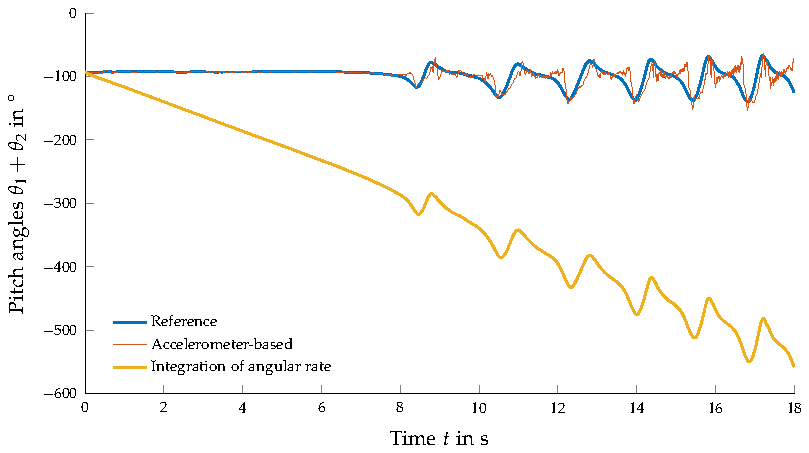
\includegraphics[width=\textwidth]{Tikz/experiment_1.tikz}
	\caption{Pitch angle of the right shank with respect to the $x$-axis, obtained by the projection of the gravity vector and by integrating the angular rate, in comparison to the reference.}
	\label{fig:experiment_1}
\end{figure}
  
  \item \textsc{kalman filter:} The third algorithm fused the orientation angle based on the projection of the gravity vector with the angle based on the integration of the angular rate measured with the gyroscope in a classical Kalman filter, without taking the motion intensity into account \cite{olivares_vicente_gaitwatch_2013}. The angles of the thigh and shank are estimated independently. The result in comparison with the projection of the gravity vector alone is depicted in Figure \ref{fig:experiment_2}.

\begin{figure}
	\centering
	\setlength\figureheight{7cm} 
	\setlength\figurewidth{\textwidth}
	\tikzsetnextfilename{experiment_2}
	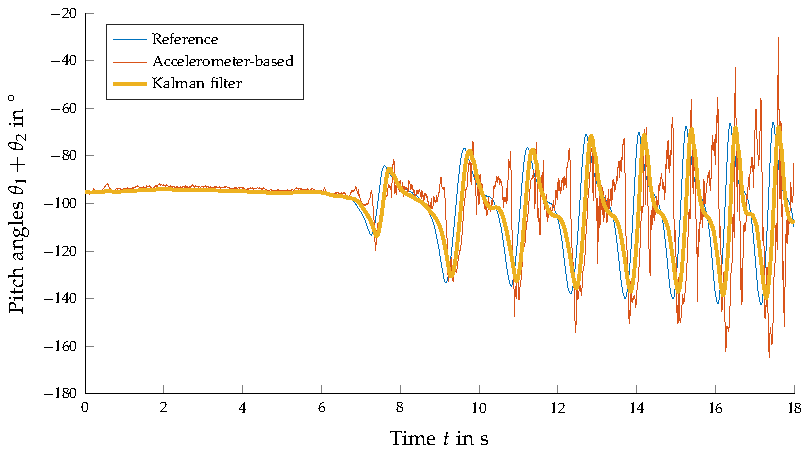
\includegraphics[width=\textwidth]{Tikz/experiment_2.tikz}
	\caption{Pitch angle of the right shank with respect to the $x$-axis, obtained by the projection of the gravity vector and by sensor fusion of accelerometer and gyroscope data in a classical Kalman filter, in comparison to the reference.}
	\label{fig:experiment_2}
\end{figure}
  
%  \item \textsc{gated kalman filter:} This algorithm extended the aforementioned classic Kalman filter by setting the measurement noise covariance according to the motion intensity \cite{olivares_vicente_gaitwatch_2013} and was already described in detail in Section \ref{sec:state_of_the_art_kalman}. Figure \ref{fig:experiment_3} compares the gated Kalman filter with the classical Kalman filter and the accelerometer-based approach.

%\begin{figure}
%	\centering
%	\setlength\figureheight{7cm} 
%	\setlength\figurewidth{\textwidth}
%	\tikzsetnextfilename{experiment_3}
%	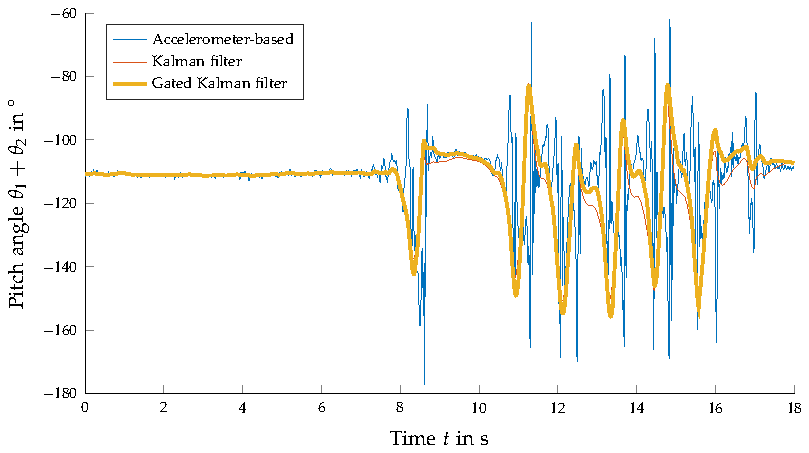
\includegraphics[width=\textwidth]{Tikz/experiment_3.tikz}
%	\caption{Pitch angle of the right shank with respect to the $x$-axis obtained by the projection of the gravity vector, gated Kalman filtering, in comparison to the reference.}
%	\label{fig:experiment_3}
%\end{figure}

  \end{itemize}

In tandem with the orientation angles estimated with the algorithms mentioned above, an angle estimate based on a Qualisys\textsuperscript{\textregistered} motion capture system served as a reference. The Qualisys\textsuperscript{\textregistered} uses high-speed cameras in combination with optical markers placed on the legs, as depicted in Figure \ref{fig:marker_placement}. From the recorded trace of the markers in space the reference angles of the thighs and shanks could be computed using an existing algorithm.

\begin{figure}
\centering
	\begin{tikzpicture}[auto, thick, node distance=3cm,>=latex']
    \pgftext{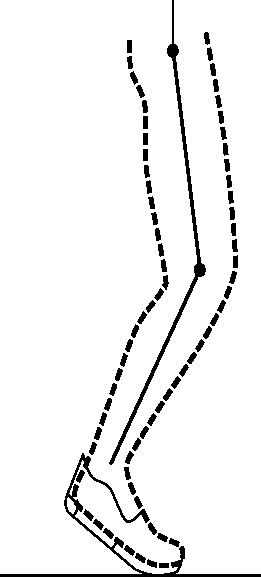
\includegraphics[width=3.5cm]{Figures/sensors_on_leg}} at (0pt,0pt);
    \node [] (a) at (-4.4, -2) {};
    \node [] (b) at (-4.5, 0.1) {};
    \node [] (c) at (4.45, 3.3) {};
    \draw[fill=black] (1.4, 2.2) circle (4pt) node[label={[label distance=0mm]0:Marker $1$}]{};
    \draw[fill=black] (1.55, 0.7) circle (4pt) node[label={[label distance=0mm]0:Marker $2$}]{};
    \draw[fill=black] (1.34, -0.4) circle (4pt) node[label={[label distance=0mm]0:Marker $3$}]{};
    \draw[fill=black] (0.4, -1.9) circle (4pt) node[label={[label distance=0mm]0:Marker $4$}]{};
\end{tikzpicture}
\caption{Human leg with optical markers, from \cite{tao_gait_2012}.} \label{fig:marker_placement}
\end{figure} 

\section{Theoretical Design}\label{sec:theoretical_design}

This section maps the theoretical design of the system proposed by \citeauthor{bennett_motion_2014} in \cite{bennett_motion_2014} to the existing GaitWatch system. It states the assigned coordinate frames and the conventions regarding rotations about their axes. Furthermore, it presents the kinematic model used to improve the angle estimates and the extended Kalman filter algorithm with its underlying state-space model in detail.

\subsection{Kinematic Model}

\begin{figure}
\centering
\begin{tikzpicture}[auto, thick,>=latex']
	\node [draw, rectangle, minimum height=1.6cm, minimum width=1.6cm, pattern=north west lines] at (0,0) (solid) {};

    \node [draw,  fill=white, very thick, rectangle, rounded corners=3pt, minimum height=3.7cm, minimum width=1cm, align=center, rotate around={30:(0,0)}] at (0.7, -1.25) (link1) {};
    \node [draw, thick, fill=gray, rounded corners=2pt, rectangle, minimum height=0.8cm, minimum width=0.45cm, align=center, rotate around={30:(0, 0)}, label={[label distance=0.18cm]335:IMU $1$}] at (0.98, -1.7) (sensor1) {};
    
    \node [draw, fill=white, very thick, rectangle, rounded corners=3pt, minimum height=3.6cm, minimum width=0.6cm, align=center, rotate around={145:(0,0)}] at (0.6, -3.7) (link2) {};
    \node [draw, thick, fill=gray, rounded corners=2pt, rectangle, minimum height=0.8cm, minimum width=0.45cm, align=center, rotate around={145:(0, 0)}, label={right:IMU $2$}] at (0, -4.56) (sensor2) {};
    
    \node[coordinate] (X) at (2.5,0) {};
    \node[coordinate] (Y) at (0,-2.5) {};
    \node[coordinate] (O) at (-0, 0) {};
    
    \draw[->] (O) -- node[name=x] {$x$}(X);
    \draw[->] (O) -- node[pos=0.6, name=y, label={left:$z$}] {}(Y);
    
    \draw[->] (0, -4.56) -- node[name=x_2] {$X_2$}(1.5, -5.6);
    \draw[->] (0, -4.56) -- node[name=x_2] {$Z_2$}(-1.1, -6.1);
   
    \draw[dotted] (O) -- (2.5,-4.3);
    \draw[fill=white] (0,0) circle (4pt);
    \draw[fill=black] (0,0) circle (1pt) node[label={[label distance=-1.2mm]180:$y$}]{};
    \draw (1.45, -2.5) circle (4pt);
    
    \draw[-stealth] (1.2,-1) arc (300:355:1.2);
    \draw[-stealth] (0.8,-4.1) arc (240:303:1.4);
    
    \node at (1.3, -0.4) (angle1) {$\theta_1$};
    \node at (1.5, -3.7) (angle1) {$\theta_2$};
\end{tikzpicture}
\caption{Kinematic model of the human leg, from \cite{bennett_motion_2014}.} \label{fig:robot}
\end{figure} 


The kinematic model relates the respective angles of the thigh and shank about the hip and knee joint to the acceleration seen by the wearable sensors. When walking in a straight line, the human leg can be modelled as a two-link planar revolute robot \cite{bennett_motion_2014}. Then, thighs and shanks remain in a single plane, which is approximately parallel to the direction of motion. As depicted in Figure \ref{fig:robot}, the revolute joints of the pendulum robot represent the hip and knee joint, and the two links the thigh and shank, respectively. The origin of the inertial world frame is located at the base of link $1$, the upper of both links. The $x$-axis points forward, the $y$-axis points out from the hip to the right, and the $z$-axis points down. This configuration follows the right-hand rule, which can also be used to determine the sense of rotation around the axes. The pitch angle $\theta_1$ is measured with respect to the $x$-axis, and the pitch angle $\theta_2$ of link $2$ with respect to link $1$.


The \glspl{IMU} placed on the thighs and shanks measured the angular velocity around the $y$-axis and the linear acceleration along the $x$ and $z$-axis, respectively. According to \citeauthor{spong2005robot} \cite{spong2005robot}, the $x$ and $z$-displacement and its derivatives in the world frame are as follows:

\begin{align}
  x &= + l_1 \cos(\theta_1) + l_2 \cos(\theta_1 + \theta_2) \\
  \dot{x} &= -l_1 \dot{\theta}_1 \sin(\theta_1) - l_2 (\dot{\theta}_1 + \dot{\theta}_2) \sin(\theta_1 + \theta_2) \\
  \ddot{x} &= -l_1 [\dot{\theta}^2_1 \cos(\theta_1) + \ddot{\theta}_1 \sin(\theta_1)] - l_2 [(\dot{\theta}_1 + \dot{\theta}_2)^2 \cos(\theta_1 + \theta_2) \nonumber \\ 
  &\mathrel{\phantom{=}} + (\ddot{\theta}_1 + \ddot{\theta}_2) \sin(\theta_1 + \theta_2)] \label{eq:acc_x} \\
  \nonumber \\
  z &= -l_1 \sin(\theta_1) - l_2 \sin(\theta_1 + \theta_2) \\
  \dot{z} &= -l_1 \dot{\theta}_1 \cos(\theta_1) - l_2 (\dot{\theta}_1 + \dot{\theta}_2) \cos(\theta_1 + \theta_2) \\
  \ddot{z} {}&= -l_1 [\ddot{\theta}_1 \cos(\theta_1) - \dot{\theta}^2_1 \sin(\theta_1)] - l_2 [(\ddot{\theta}_1 + \ddot{\theta}_2) \cos(\theta_1 + \theta_2) \nonumber \\ 
  &\mathrel{\phantom{=}} - (\dot{\theta}_1 + \dot{\theta}_2)^2 \sin(\theta_1 + \theta_2)] \label{eq:acc_y}
\end{align}

\noindent
in which $l_1$ and $l_2$ are the lengths of the two links, respectively. Plugging the \emph{a priori} estimates of the angles $\theta_1$ and $\theta_2$ and their derivatives, i.\,e. the angular rates $\omega_1$ and $\omega_2$, and the angular accelerations $\alpha_1$ and $\alpha_2$, obtained with the EKF described in Section \ref{sec:EKF_model}, into Equations \ref{eq:acc_x} and \ref{eq:acc_y}, we can estimate the respective motion-based acceleration components $a_x$ and $a_z$ in $x$ and $z$-direction that sensor $2$ will see in the world coordinate frame. Written as a function of the state variables of the extended Kalman filter, Equations \ref{eq:acc_x} and \ref{eq:acc_y} yield

\begin{align}
  a_x &= -l_1 [\omega^2_1 \cos(\theta_1) + \alpha_1 \sin(\theta_1)] - l_2 [(\omega_1 + \omega_2)^2 \cos(\theta_1 + \theta_2) \nonumber \\ 
  &\mathrel{\phantom{=}} + (\alpha_1 + \alpha_2) \sin(\theta_1 + \theta_2)] \label{eq:acc_x_state} \\
  \nonumber \\
  a_z {}&= -l_1 [\alpha_1 \cos(\theta_1) - \omega^2_1 \sin(\theta_1)] - l_2 [(\alpha_1 + \alpha_2) \cos(\theta_1 + \theta_2) \nonumber \\ 
  &\mathrel{\phantom{=}} - (\omega_1 + \omega_2)^2 \sin(\theta_1 + \theta_2)] \label{eq:acc_y_state}
\end{align}

The orientation of the sensor frames at rest are different from the world frame and dynamic when the pendulum is in motion. In order to transform the values from the world frame to the dynamic body frame of \gls{IMU} $2$, which is depicted in Figure \ref{fig:robot}, we used the transformation matrix $\mathbf{T}_y(\theta)$ from Equation \ref{eq:transformation_matrices}. The body frame of sensor two is not aligned with the world frame for $\theta_1 = \theta_2 = 0$. Thus, in order to align both frames, an offset of $90^{\circ}$ is required. With $\theta = \theta_1 + \theta_2 + 90^{\circ}$, this yields

\begin{equation}
\begin{split}
\mathbf{T}_y(\theta_1 + \theta_2 + 90^{\circ}) &= \left[ \begin{smallmatrix}
    \cos (\theta_1 + \theta_2 + 90^{\circ}) \; & 0 \; & -\sin (\theta_1 + \theta_2 + 90^{\circ}) \\
    0 \; & 1 \; & 0 \\
    \sin (\theta_1 + \theta_2 + 90^{\circ}) \; & 0 \; & \cos (\theta_1 + \theta_2 + 90^{\circ})
    \end{smallmatrix} \right] \\
    &= \left[ \begin{smallmatrix}
    -\sin (\theta_1 + \theta_2) \; & 0 \; & -\cos (\theta_1 + \theta_2) \\
    0 \; & 1 \; & 0 \\
    \cos (\theta_1 + \theta_2) \; & 0 \; & -\sin (\theta_1 + \theta_2)
    \end{smallmatrix} \right] \,.
\end{split}
\end{equation}

\noindent
According to Equation \ref{eq:transformation}, the rotated radial and tangential components of the motion-based acceleration estimates in the body frame of accelerometer $2$, $A_{X_2}$ and $A_{Z_2}$, are found by pre-multiplying the transformation matrix with the acceleration vector in the world frame, constituted of the results of Equations \ref{eq:acc_x_state} and \ref{eq:acc_y_state}.

\begin{equation}
  \mathbf{a} = \begin{bmatrix}
  	a_{X_2} \\
  	a_{Y_2} \\
  	a_{Z_2}
  \end{bmatrix} = \mathbf{T}_y(\theta_1 + \theta_2 + 90^{\circ}) \begin{bmatrix}
  	a_x \\
  	0 \\
	a_z
  \end{bmatrix} \|\mathbf{g}\|^{-1}
\end{equation}

\noindent
The axial component $A_{Y_2}$ is zero, since the leg is assumed to be oriented perpendicular to the earth's surface and thus the gravity vector $\mathbf{g}$ is perpendicular to the $y$-axis. The term $\|\mathbf{g}\|^{-1}$ normalises the motion-based acceleration estimate to gravity, where $\|\mathbf{g}\|$ denotes the magnitude of gravity. 

Then, the motion based radial and tangential acceleration components are subtracted from the sensor readings $a_{X_1m}$ and $a_{Z_1m}$, which leaves an estimate of the gravity based acceleration $\mathbf{g}$ that acts on the sensor:

\begin{equation}
\mathbf{g} = \begin{bmatrix}
    g_x \\
    g_y \\
    g_z 
    \end{bmatrix} \approx 
    \begin{bmatrix}
    a_{X_2m} \\
    0 \\
    a_{Z_2m} 
    \end{bmatrix} -
    \begin{bmatrix}
    a_{X_2} \\
    0 \\
    a_{Z_2} 
    \end{bmatrix}\,.
\end{equation}

\noindent
The angle estimate of the shank with respect to the $x$-axis, based on the projection of the gravity vector on the axes of the accelerometer, is then

\begin{equation}
  \theta_1 + \theta_2 = \mbox{atan}2(g_z, g_x)-180^{\circ}\,.
\end{equation}

\noindent
This improved angle estimate is then fused with the estimate based on the integration of the angular rate measured with the gyroscope, in order to reduce the estimation error due to gyroscope drift.

\subsection{The Extended Kalman Filter} \label{sec:EKF_model}

\subsubsection{The State-Space Model}

The state-space model of the extended Kalman filter is given by the state vector $\mathbf{x} \in \mathbb{R}^{n}$, with $n=10$,

\begin{equation} \label{eq:state_vector}
  \mathbf{x} = \begin{bmatrix}
  	x, & z, & \theta_1, & \omega_1, & \alpha_1, & \theta_2, & \omega_2, & \alpha_2, & \beta_1, & \beta_2
  \end{bmatrix}^T\,,
\end{equation}

\noindent
where $x$ and $y$ correspond to the horizontal and vertical position of the end of link $2$ with respect to the origin of the world frame, i.\,e. the hip joint. $\theta_1$ is the angle, $\omega_1$ the angular velocity, and $\alpha_1$ the angular acceleration of the first joint, respectively. The corresponding values for the second link are $\theta_2$, $\omega_2$, and $\alpha_2$. The biases of the gyroscopes in the first and the second IMU are $\beta_1$ and $\beta_2$, respectively. They are assumed to be constant or slowly time-varying.

The measurement vector $\mathbf{z} \in \mathbb{R}^m$, with $m = 4$, is given by

\begin{equation} \label{eq:measurement_vector}
  \mathbf{z} = \begin{bmatrix} z_1 \\ z_2 \\ z_3 \\ z_4 \end{bmatrix} = \begin{bmatrix}
  	\omega_1 + \beta_1, & \omega_1 + \omega_2 + \beta_1 + \beta_2, & \theta_1, & \theta_1 + \theta_2
  \end{bmatrix}^T + \mathbf{v}\,,
\end{equation}
 
\noindent
where $\mathbf{v}$ is the random measurement noise process, modelled as zero-mean, Gaussian white noise. The element $z_1$ represents the measurement of the first link angular velocity, which is the sum of the first link rotation and the gyroscope $1$ bias. The element $z_2$ represents the measurement of the second link angular velocity, which is the sum of the first and second link rotation and the bias of gyroscope $1$ and gyroscope $2$. Finally, the element $z_3$ is the angle estimate of the first accelerometer and the element $z_4$ the angle estimate of the second accelerometer, which will see the angular displacement of both links.

According to  \citeauthor{rowell2002state} \cite{rowell2002state}, the plant dynamics of a system can be expressed as a set of $n$ coupled first-order ordinary differential equations, known as the \emph{state equations}. The modelled system is governed by the \emph{non-linear} first-order ordinary differential equations

\begin{equation} \label{eq:state_vector_derivative}
  \dot{\mathbf{x}} = \mathbf{f}(\mathbf{x}, t) + \mathbf{w} = \left[\begin{smallmatrix}
  -l_1 \omega_1 \sin(\theta_1)  - l_2 (\omega_1 + \omega_2) \sin(\theta_1 + \theta_2) \\
  -l_1 \omega_1 \cos(\theta_1)  - l_2 (\omega_1 + \omega_2) \cos(\theta_1 + \theta_2) \\ \omega_1 \\ \alpha_1 \\ 0 \\ \omega_2 \\ \alpha_2 \\ 0 \\ 0 \\ 0
  \end{smallmatrix}\right] + \mathbf{w}\,,
\end{equation}

\noindent
where $\dot{\mathbf{x}}$ consists of the component-wise time derivatives of the state vector $\mathbf{x}$, expressed in terms of the state variables $x_1(t), \dots, x_n(t)$. Its elements are given by

\begin{equation}
  \dot{x}_i = f_i(x_1(t), \dots, x_n(t), t) + w_i = \frac{dx_i}{dt} + w_i\,, \quad i = 1, \dots, n\,.
\end{equation}

\noindent
The noise term $\mathbf{w}$, modelled as zero-mean, Gaussian white noise again represents the uncertainty in the model. Given this \emph{state-space representation}, the system state at any instant may be interpreted as a point in an $n$-dimensional state space whose axes are the state variables. The dynamic state response $\mathbf{x}(t)$ can be interpreted as a trajectory traced out in the state space. The system described by Equation \ref{eq:state_vector_derivative} is \emph{time-invariant}, since it does not depend explicitly on time. Thus, we may leave out the $t$ and write from now on $\mathbf{f}(\mathbf{x}) = \mathbf{f}(\mathbf{x}, t)$.

For a \emph{linear} system in state-space form given by

\begin{equation}\label{eq:linear_continuous}
  \dot{\mathbf{x}} = \mathbf{F} \mathbf{x}\,,
\end{equation}

\noindent
with a time-invariant \emph{system dynamics matrix} $\mathbf{F}$ there is a \emph{state transition matrix} $\bm{\Phi}(t-t_0)$ that propagates the state of the system forward from any time $t_0$ to a time $t$, according to

\begin{equation}
  \mathbf{x}(t) = \bm{\Phi}(t-t_0) \mathbf{x}(t_0)\,.
\end{equation}

\noindent
The solution to the system described by Equation \ref{eq:linear_continuous} is 

\begin{equation}
  \mathbf{x}(t) = e^{\mathbf{F}(t-t_0)} \mathbf{x}(t_0)\,,
\end{equation}

\noindent
where $\mathbf{x}(t_0)$ is an integration constant. As outlined in \cite{zarchan2009fundamentals}, the state transition matrix can be found by a Taylor-series expansion of $e^{\mathbf{F}(t-t_0)}$,

\begin{equation}
\begin{split}
  \bm{\Phi}(t-t_0) = e^{\mathbf{F}(t-t_0)} &= \sum_{k=0} ^ {\infty} \frac {\mathbf{F}^{n} [t-t_0]^n}{k!} \\
  &= \mathbf{I}_n + \mathbf{F}[t-t_0] \\ 
  & \mathrel{\phantom{= \mathbf{I}_n}} + \frac{\mathbf{F}^2 [t-t_0]^2}{2!} +\frac{\mathbf{F}^{3} [t-t_0]^3}{3!} + \cdots\,,
\end{split}
\end{equation}
 
\noindent
where $\mathbf{I}_n \in \mathbb{R}^{n \times n}$ is the identity matrix. Truncating the Taylor series after the first order terms yields the \emph{linear approximation} of the fundamental matrix:

\begin{equation}
  \bm{\Phi}(t-t_0) \approx \mathbf{I}_n + \mathbf{F}[t-t_0]\,.
\end{equation}

\noindent
The discrete fundamental matrix that propagates the state of the system forward from time step $k$ to $k+1$ can be found by substituting $T_s$ for $t-t_0$, which yields

\begin{equation}
  \bm{\Phi}_{k} = \bm{\Phi}(T_s) \approx \mathbf{I}_{n} + \mathbf{F} T_s\,,
\end{equation}

\noindent
where $T_s$ is the sampling period. In the \emph{linear} case $\bm{\Phi}_{k}$ is constant.

Because the state equations of our system are \emph{non-linear}, a first-order approximation of the system dynamics matrix $\mathbf{F}$ is used, given by the Jacobian of $\mathbf{f}(\mathbf{x})$

\begin{equation}
\begin{split}
\mathbf{F}^{[1]}_k = \mathbf{J}_{\mathbf{f}} &= \begin{bmatrix}
    \dfrac{\partial f_1}{\partial x_1} & \cdots & \dfrac{\partial f_1}{\partial x_{n}}\\
    \vdots & \ddots & \vdots\\
    \dfrac{\partial f_{n}}{\partial x_1} & \cdots & \dfrac{\partial f_{n}}{\partial x_{n}} \end{bmatrix} \\
&=\begin{bmatrix}
  0 & 0 & A & C & 0 & E & G & 0 & 0 & 0\\
  0 & 0 & B & D & 0 & F & H & 0 & 0 & 0\\
  0 & 0 & 0 & 1 & 0 & 0 & 0 & 0 & 0 & 0\\
  0 & 0 & 0 & 0 & 1 & 0 & 0 & 0 & 0 & 0\\
  0 & 0 & 0 & 0 & 0 & 0 & 0 & 0 & 0 & 0\\
  0 & 0 & 0 & 0 & 0 & 0 & 1 & 0 & 0 & 0\\
  0 & 0 & 0 & 0 & 0 & 0 & 0 & 1 & 0 & 0\\
  0 & 0 & 0 & 0 & 0 & 0 & 0 & 0 & 0 & 0\\
  0 & 0 & 0 & 0 & 0 & 0 & 0 & 0 & 0 & 0\\
  0 & 0 & 0 & 0 & 0 & 0 & 0 & 0 & 0 & 0\\
\end{bmatrix}_{\mathbf{x}=\hat{\mathbf{x}}_{k}}\,,
\end{split}
\end{equation}

\noindent
with

\begin{equation*}
  \begin{split}
  	A &= -l_1 \omega_1 \cos(\theta_1) -l_2 (\omega_1 + \omega_2) \cos(\theta_1 + \theta_2)\,, \\
  	B &= +l_1 \omega_1 \sin(\theta_1) +l_2 (\omega_1 + \omega_2) \sin(\theta_1 + \theta_2)\,, \\
  	C &= -l_1 \sin(\theta_1) -l_2 \sin (\theta_1 + \theta_2)\,, \\
  	D &= -l_1 \cos(\theta_1) - l_2 \cos (\theta_1 + \theta_2)\,, \\
  	E &= -l_2 (\omega_1 + \omega_2) \cos(\theta_1+ \theta_2)\,, \\
  	F &= +l_2 (\omega_1 + \omega_2) \sin(\theta_1+ \theta_2)\,, \\
    G &= -l_2 \sin (\theta_1 + \theta_2)\,, \\
    H &= -l_2 \cos (\theta_1 + \theta_2)\,.
  \end{split}
\end{equation*}

\noindent
The partial derivatives are evaluated at the state estimate $\hat{\mathbf{x}}_{k}$. The discrete state transition matrix must be recomputed every time step. Here the subscript $k$ denotes the state transition matrix that propagates the state at time step $k$ to time step $k+1$. It is given by 

\begin{equation}
  \bm{\Phi}^{[1]}_{k} \approx \mathbf{I}_{n} + \mathbf{F}^{[1]}_k T_s\,.
\end{equation}

\subsubsection{The Filter Algorithm} 

The estimate $\hat{\mathbf{x}}_{k-1}$ can be propagated forward to the \emph{a priori} estimate $\hat{\mathbf{x}}^{-}_k$ by integrating the \emph{non-linear} differential equations at each sampling interval. Applying Euler integration Equation \ref{eq:apriori_estimate_extended} yields

\begin{equation}\label{eq:apriori_estimate_extended_model}
\begin{split}
	\hat{\mathbf{x}}^{-}_k &= \bm{\phi}_{k-1}(\hat{\mathbf{x}}_{k-1}, 0) \\
	&= \hat{\mathbf{x}}_{k-1} + \mathbf{f}(\hat{\mathbf{x}}_{k-1})T_s\,, 
\end{split} 
\end{equation}

\noindent
where $T_s$ is the integration interval. The control input $\mathbf{u}_k$ is equal to zero since the system does not have any inputs. A higher-order numerical integration procedure would not improve the \emph{a priori} estimate since the function $\mathbf{f}(\mathbf{x})$ is constant over time.

The relation between the states and the measurements is \emph{linear}, according to Equation \ref{eq:time_dynamical_system_measurement}. The measurement matrix $\mathbf{H} \in \mathbb{R}^{3 \times 10}$ is given by 

\begin{equation}
\mathbf{H} = \begin{bmatrix}
  0 & 0 & 0 & 1 & 0 & 0 & 0 & 0 & 1 & 0\\
  0 & 0 & 0 & 1 & 0 & 0 & 1 & 0 & 1 & 1\\
  0 & 0 & 1 & 0 & 0 & 0 & 0 & 0 & 0 & 0 \\
  0 & 0 & 1 & 0 & 0 & 1 & 0 & 0 & 0 & 0\\
\end{bmatrix}\,.
\end{equation}

The process noise covariance matrix $\mathbf{Q} \in \mathbb{R}^{10 \times 10}$ is constant and given by

\begin{equation}
\begin{split}
\mathbf{Q} &= \begin{bmatrix}
 \operatorname{Cov}(w_1,w_1) & \operatorname{Cov}(w_1,w_2) & \cdots & \operatorname{Cov}(w_1,w_n) \\ \\
 \operatorname{Cov}(w_2,w_1) & \operatorname{Cov}(w_2,w_2) & \cdots & \operatorname{Cov}(w_2,w_n) \\ \\
 \vdots & \vdots & \ddots & \vdots \\ \\
 \operatorname{Cov}(w_n,w_1) & \operatorname{Cov}(w_n,w_2) & \cdots & \operatorname{Cov}(w_n,w_n)
\end{bmatrix} \\
&= \begin{bmatrix}
  \sigma^2_d & 0 & 0 & 0 & 0 & 0 & 0 & 0 & 0 & 0\\
  0 & \sigma^2_d & 0 & 0 & 0 & 0 & 0 & 0 & 0 & 0\\
  0 & 0 & \frac{\sigma^{18}_{\theta_1}}{9} & \frac{\sigma^8_{\theta_1}}{4} & \frac{\sigma^{10}_{\theta_1}}{5} & 0 & 0 & 0 & 0 & 0\\
  0 & 0 & \frac{\sigma^8_{\theta_1}}{4} & \frac{\sigma^6_{\theta_1}}{3} & \frac{\sigma^4_{\theta_1}}{2} & 0 & 0 & 0 & 0 & 0\\
  0 & 0 & \frac{\sigma^{10}_{\theta 1}}{5} & \frac{\sigma^4_{\theta_1}}{2} & \sigma^2_{\theta_1} & 0 & 0 & 0 & 0 & 0\\
  0 & 0 & 0 & 0 & 0 & \frac{\sigma^{18}_{\theta_2}}{9} & \frac{\sigma^8_{\theta_2}}{4} & \frac{\sigma^{10}_{\theta_2}}{5} & 0 & 0\\
  0 & 0 & 0 & 0 & 0 & \frac{\sigma^8_{\theta_2}}{4} & \frac{\sigma^6_{\theta_2}}{3} & \frac{\sigma^4_{\theta_2}}{2} & 0 & 0\\
  0 & 0 & 0 & 0 & 0 & \frac{\sigma^{10}_{\theta_2}}{5} & \frac{\sigma^4_{\theta_2}}{2} & \sigma^2_{\theta_2} & 0 & 0\\
  0 & 0 & 0 & 0 & 0 & 0 & 0 & 0 & \sigma^2_{\beta} & 0\\
  0 & 0 & 0 & 0 & 0 & 0 & 0 & 0 & 0 & \sigma^2_{\beta}\\
\end{bmatrix}\,.
\end{split}
\end{equation}

\noindent
The diagonal elements represent the respective variances of the elements $w_1, \dots, w_n$ of the process noise vector $\mathbf{w}$, due to the relation $\operatorname{Cov}(w_i,w_i) = \operatorname{Var}(w_i)$. The other elements are the covariances of all possible pairs of the random variables of the process noise vector. The noise processes interfering with the state variables $x$ and $y$, and $\beta_1$ and $\beta_2$, respectively, were modelled as independent. In contrast, the covariances of the noise components interfering with the state variables $\theta_i, \omega_i, \alpha_i, i \in {1, 2}$, which account for the block-diagonal structure, reflect a random walk process, that is, the integration of a signal perturbed by Gaussian white noise. A detailed derivation of the form of the elements is found in \cite{Kelly_1994_random}. The parameters $\sigma_d, \sigma_{\theta_1}, \sigma_{\theta_2},$ and $\sigma_{\beta}$ were found by an optimiser, which is described in Section \ref{sec:preparation}.

The measurement noise covariance matrix $\mathbf{R} \in \mathbb{R}^{4 \times 4}$, is given by

\begin{equation}
\mathbf{R} = \begin{bmatrix}
  \sigma^2_1 & 0 & 0 & 0\\
  0 & \sigma^2_2 & 0 & 0\\
  0 & 0 & \sigma^2_3 & 0\\
  0 & 0 & 0 & \sigma^2_4
\end{bmatrix}\,,
\end{equation}

The parameters $\sigma^2_1$ and $\sigma^2_2$ are constant. They are determined by computing the sample variance of the measurement data during an initialisation stage of $T_{\text{init}} = 2$\,s seconds, while the subject stands still. The variance of a finite data set with $n$ samples $x_1, x_2, \dots, x_n$ is given by

\begin{equation}
  \sigma^2 = \frac{1}{n-1} \sum_{k=1}^n (x_k - \mu)^2, {\rm \ \ where\ \ } \mu = \frac{1}{n} \sum_{k=1}^n x_k\,.
\end{equation}

\noindent
with

\begin{equation}
  n = T_{\text{init}} f_s\,.
\end{equation}


\noindent
The variances $\sigma^2_3$ and $\sigma^2_4$ of the accelerometer-based angle estimates were found by the optimiser and were set dynamically at each time step $k$, based on the motion intensity. It toggles between $\sigma_s$ and $\sigma_f$, according to slow or fast motion, distinguished by a marker signal $m_k$:

\begin{equation}
  \sigma^2_3 = \begin{cases}
  	\sigma^2_{3s} & \quad m_k = 0 \\
  	\sigma^2_{3f} & \quad m_k = 1
  \end{cases}\,.
\end{equation}

\begin{equation}
  \sigma^2_4 = \begin{cases}
  	\sigma^2_{4s} & \quad m_k = 0 \\
  	\sigma^2_{4f} & \quad m_k = 1
  \end{cases}\,.
\end{equation}

\noindent
In order to determine the marker signal we used the long term spectral detector \gls{LTSD} developed in \cite{olivares_vicente_gaitwatch_2013}, which distinguishes between fast and slow motion by computing the long term spectral envelope of the signal. The output of the LTSD is a marker signal which value toggles between $1$ and $0$.

\subsubsection{Summary of the Entire Filter Algorithm}

The state estimates are computed recursively according to the \emph{time update} Equations \ref{eq:apriori_error_cov_extended}, \ref{eq:apriori_estimate_extended_model} and the \emph{measurement update} Equations \ref{eq:aposteriori_estimate}, \ref{eq:Kalman_gain}, and \ref{eq:aposteriori_error_cov}. The entire computation steps of the recursive filter algorithm are summarised in Figure \ref{fig:entire_filter_algorithm}. Listing \ref{lis:filter} in the appendix shows the \textsc{Matlab}\textsuperscript{\textregistered} implementation of the filter function.

\tikzstyle{block} = [draw, rectangle, thick, 
    minimum height=1.5cm, minimum width=10cm]
\tikzstyle{output} = [coordinate]

\begin{figure}
\centering
\begin{tikzpicture}[scale=0.95, every node/.style={transform shape}, auto, rounded corners=1pt, node distance=5cm,>=latex']
    
\node [block, align=center] (init) {Initialisation of parameters \\[2mm]  $\mathbf{x}_{0}, \mathbf{P}_{0}, \mathbf{H}, \mathbf{Q}, \mathbf{R}_{0},$};
\node [block, align=center, below of=init, node distance=3.8cm] (predict) {\emph{Time update} \\[2mm] Compute fundamental matrix: \\ $\bm{\Phi}^{[1]}_{k-1} \approx \mathbf{I}_{n} + \mathbf{F}_{k-1} T_s$ \\ Compute \emph{a priori} estimate: \\ $\hat{\mathbf{x}}^{-}_k = \hat{\mathbf{x}}_{k-1} + \mathbf{f}(\hat{\mathbf{x}}_{k-1})T_s$ \\ Compute \emph{a priori} error covariance: \\ $\mathbf{P}^-_{k} = \bm{\Phi}^{[1]}_{k-1} \mathbf{P}_{k-1} \bm{\Phi}^{[1]T}_{k-1} + \mathbf{Q}_{k-1}$};
\node [block, align=center, below of=predict, node distance=6.65cm] (measurement) {\emph{Correct sensor readings} \\[2mm] Compute acceleration due to motion: \\ $a_x = -l_1 [\omega^2_1 \cos(\theta_1) + \alpha_1 \sin(\theta_1)] - l_2 [(\omega_1 + \omega_2)^2$ \\ $\mathrel{\phantom{}}\cdot \cos(\theta_1 + \theta_2) + (\alpha_1 + \alpha_2) \sin(\theta_1 + \theta_2)]$ \\ $a_z = -l_1 [\alpha_1 \cos(\theta_1) - \omega^2_1 \sin(\theta_1)] - l_2 [(\alpha_1 + \alpha_2)$ \\ $\mathrel{\phantom{=ii}} \cdot \cos(\theta_1 + \theta_2) + (\omega_1 + \omega_2)^2 \sin(\theta_1 + \theta_2)]$ \\ Compute gravity estimate: \\ $\mathbf{g} \approx 
    \left[ \begin{smallmatrix}
    a_{X_2m} \\
    0 \\
    a_{Z_2m} 
    \end{smallmatrix} \right] -
    \mathbf{T}_y(\theta_1 + \theta_2 + 90^{\circ}) \left[ \begin{smallmatrix}
  	a_x \\
  	0 \\
	a_z
  \end{smallmatrix} \right] \|\mathbf{g}\|^{-1}$ \\ Compute corrected angle estimate: \\ $\theta_1 + \theta_2 = \mbox{atan}2(g_z, g_x)-180^{\circ}$ \\ Set measurement covariances: \\ $\sigma^2_3 = \begin{cases}
  	\sigma^2_{3s} & \quad m_k = 0 \\
  	\sigma^2_{3f} & \quad m_k = 1
  \end{cases}\,, \quad \sigma^2_4 = \begin{cases}
  	\sigma^2_{4s} & \quad m_k = 0 \\
  	\sigma^2_{4f} & \quad m_k = 1
  \end{cases}$};
\node [block, align=center, below of=measurement, node distance=6.6cm] (update) {\emph{Measurement update} \\[3mm] Compute Kalman gain: \\ $\mathbf{K}_{k} = \mathbf{P}^-_k \mathbf{H}^T_k[\mathbf{H}_k \mathbf{P}^-_k \mathbf{H}^T_k + \mathbf{R}_k]^{-1}$ \\ Compute \emph{a posteriori} estimate: \\ $\hat{\mathbf{x}}_k = \hat{\mathbf{x}}^-_k + \mathbf{K}_{k}[\mathbf{z}_k-\mathbf{H}_{k}\hat{\mathbf{x}}^-_k]$ \\ Update error covariance: \\ $\mathbf{P}_{k} = [\mathbf{I} - \mathbf{K}_{k}\mathbf{H}_{k}]\mathbf{P}^-_{k}$};
\node [output, below of=update, node distance=3.2cm, name=output] {Output};
\node [output, below of=update, node distance=2.68cm, name=help1] {};
\node [output, right of=help1, node distance=5.6cm, name=help2] {};
\node [output, below of=init, node distance=1.18cm, name=help4] {};
\node [output, right of=help4, node distance=5.6cm, name=help3] {};

\draw [draw,-stealth, thick, align=left] (init) -- (predict);
\draw [draw,-stealth, thick, align=left] (predict) -- (measurement);
\draw [draw,-stealth, thick, align=left] (measurement) -- (update);
\draw [draw,-stealth, thick, align=left] (update) -- node [label={left:Output}]{} (output);
\draw [draw,-stealth, thick] (help1) -- (help2) -- (help3) -- (help4);
\end{tikzpicture}
\caption{Entire computation steps of the recursive filter algorithm.} \label{fig:entire_filter_algorithm}
\end{figure}


\section{Experiments}

The extended Kalman filter was tested and its results were compared to the existing classical Kalman filter and the reference signal, by interrelating the RMSE of each method. The orientation algorithms were applied to movement data from a real subject. These data were gathered at the Department of Neurology of the Klinikum Großhadern in Munich, while the subject performed the following trial.

\subsection{Data Collection Protocol}

The subject stood on a treadmill wearing the GaitWatch system on its body. Then, the GaitWatch record was started and shortly afterwards the treadmill was turned on. After a variable time, depending on the treadmill speed and the walking distance, first the treadmill was switched off, and then the GaitWatch records. The trial was performed at walking speeds of $\unitfrac[2]{km}{h}$, $\unitfrac[4]{km}{h}$, and $\unitfrac[6]{km}{h}$.

\subsection{Initial Conditions}\label{sec:initial_cond}

Each trial began with the subject standing still and it was assumed that the subject's legs were fully stretched. This leads to the following initial state estimates:

\begin{equation}
\begin{matrix}
	\begin{split}
	  x &= 0\,\mbox{m}\,, \\
	  \theta_1 &= -90^{\circ}\,, \\
	  \omega_1 &= 0\, ^{\circ}/\mbox{s} \,, \\
	  \beta_1 &= \mu_1\, ^{\circ}/\mbox{s} \,, \\
	  \alpha_1 &= 0\, ^{\circ}/\mbox{s}^2\,, 
\end{split} \qquad \quad
    \begin{split}
   	  z &= -(l_1+l_2)\,\mbox{m}\,, \\
	  \theta_2 &= 0\,^{\circ}\,, \mathrel{\phantom{90^{\circ}}}\\
	  \omega_2 &= 0\, ^{\circ}/\mbox{s} \,, \\
	  \beta_2 &= \mu_2\, ^{\circ}/\mbox{s} \,, \\
	  \alpha_2 &= 0\, ^{\circ}/\mbox{s}^2\,,  
\end{split}
\end{matrix} \\
\end{equation}

\noindent
where $\mu_1$ and $\mu_2$ are the mean values of the gyroscope signals collected during the initial $T_{\text{init}} = 2\,\mbox{s}$ of the rest period before the subject started moving. The mean value is given by

\begin{equation}
  \mu = \frac{1}{n} \sum_{k=1}^{n}{\omega_k}\,, \quad n = T_{\text{init}} f_s\,,
\end{equation}

\noindent
where $\omega_k$ is the angular velocity at instant $k$ and $f_s$ the sampling frequency.

The initial error covariance matrix was the identity matrix, $\mathbf{P}_0 = \mathbf{I}_{10} \in \mathbb{R}^{10\times10}$. Its diagonal elements, that is, the variances of the initial state estimates, represent the confidence in the knowledge about the initial state of the system and is crucial for the convergence of the filter. Unlike the initial error covariance matrix of the classical Kalman filter, it may cause the filter to diverge, in case the confidence in the estimates is too small. Equally, too vague initial state estimates can cause the filter to diverge.

\subsection{Test Preparation}\label{sec:preparation}

To test the filter algorithm and compare it with the existing classical Kalman filter, a parameter optimiser was implemente. Based on the optimal set of parameters for a given signal, we compared the newly implemented filter algorithm against the classical Kalman filter. The parameter optimisation function given by Listing \ref{lis:optimiser} called an adaptive Nelder-Mead simplex algorithm, which minimised the error function $\operatorname{E}$. Since we are interested in an accurate angle estimate of both angles and thus need parameters that optimise both angle estimates, we scalarise this multi-objective optimisation problem. Using linear scalarisation yields

\begin{equation}
\begin{split}
  \operatorname{E}(\hat{\theta}_t, \hat{\theta}_s) &= \operatorname{RMSE}_{\hat{\theta}_{t}} + \operatorname{RMSE}_{\hat{\theta}_s} \\
  &= \sqrt{\frac{\sum_{k=1}^n (\hat{\theta}_{t, k} - \theta_{t, k})^2}{n}} + \sqrt{\frac{\sum_{k=1}^n (\hat{\theta}_{s, k} - \theta_{s, k})^2}{n}}\,,
\end{split}
\end{equation}

\noindent
where $\hat{\theta}_{t,k}$ and $\hat{\theta}_{s,k}$ denote the thigh and shank angle at instant $k$, estimated by the extended Kalman filter, and $\theta_{t, k}$ and $\theta_{s, k}$ the reference angles at instant $k$, respectively. The implementation of the error function is shown in Listing \ref{lis:error_function}. The optimiser returns the parameters that minimise the error function.

\subsubsection{Parameterisation}

The parameters for the three different walking speeds in Table \ref{tab:parameters} were determined by the optimisation routines. In order to improve the legibility, all parameters are normalised to their respective units. That is, since the variance is the square of the standard deviation, they are normalised to the square of the unit of the corresponding element of the state vector as stated in Section \ref{sec:initial_cond}. For instance, the variance $\sigma^2_d$ of the displacement is normalised to $\unit[]{m^2}$.

\newcommand{\ra}[1]{\renewcommand{\arraystretch}{#1}}
\begin{table*}\centering
\ra{1.3}
\begin{tabular}{@{}lrrr@{}}\toprule
 & $\unitfrac[2]{m}{s}$ & $\unitfrac[4]{m}{s}$ & $\unitfrac[6]{m}{s}$ \\
\midrule
$\sigma^2_d$ & 10.0000 & 10.0000 & 10.0000 \\
$\sigma^2_{\theta_1}$ & 0.0514 & 0.0209 & 0.4342 \\
$\sigma^2_{\theta_2}$ & 0.0514 & 0.0209 & 0.4342 \\
$\sigma^2_{\beta}$ & 0.0011 & 0.0001 & 0.0007 \\
$\sigma^2_1$ & 2.1767 & 3.6758 & 2.7102 \\
$\sigma^2_2$ & 2.9788 & 3.2287 & 1.7409 \\
$\sigma^2_{3s}$ & 11.5799 & 7.2881 & 5.6341 \\
$\sigma^2_{3f}$ & 50.8859 & 117.2099 & 56.9627 \\
$\sigma^2_{4s}$ & 45.1827 & 24.5344 & 88.4655 \\
$\sigma^2_{4f}$ & 265.8502 & 224.4809 & 222.4782 \\
\bottomrule
\end{tabular}
\caption{Filter parameters.}
\label{tab:parameters}
\end{table*}

\subsection{Test Execution}

The testing procedure was as follows: First, the movement data of the subject were loaded into the workspace. Next, the parameters of the classical Kalman filter were optimised by an existing optimiser. Then, the parameters of the extended Kalman filter were optimised with the aforementioned EKF-optimiser. After each optimisation process the respective angle estimation was computed. Subsequently, the absolute RMSEs and the relative RMSE related to the one obtained with the classical Kalman filter were computed. Finally, the results were displayed in the console and depicted in four plots: The thigh and shank angle estimate, respectively, the RMSE comparison, and the acceleration correction. The \mbox{\textsc{Matlab}\textsuperscript{\textregistered}} code for the first data set is given in Listing \ref{lis:experiments_1}. The results are presented in the next section.

\section{Results}

The results of the experiments are presented as follows:

\begin{itemize}
  \item \textsc{thigh angles:} Comparison of the temporal courses of the pitch angles of the right thigh with respect to the $x$-axis obtained by projection of the gravity vector, classical Kalman filtering, and extended Kalman filtering, in comparison to the reference, for the three different walking speeds, depicted in Figures \ref{fig:experiment_4}, \ref{fig:experiment_8}, and \ref{fig:experiment_12}.
  \item \textsc{shank angles:} Comparison of the temporal courses of the pitch angles of the right shank with respect to the $x$-axis obtained by projection of the gravity vector, classical Kalman filtering, and extended Kalman filtering, in comparison to the reference, for the three different walking speeds, depicted in Figures \ref{fig:experiment_5}, \ref{fig:experiment_9}, and \ref{fig:experiment_13}.
  \item \textsc{rmse comparison:} Root-mean-square error comparison of angle estimations by projection of the gravity vector, classical Kalman filtering, and extended Kalman filtering, for the three different walking speeds, depicted in Figures \ref{fig:experiment_6}, \ref{fig:experiment_10}, and \ref{fig:experiment_14}.
  \item \textsc{acceleration correction:} Comparison of the accelerometer-based shank angles with respect to the $x$-axis with and without correction of the acceleration signal, for the three different walking speeds, depicted in Figures \ref{fig:experiment_7}, \ref{fig:experiment_11}, and \ref{fig:experiment_15}.
\end{itemize}

\noindent
The entire absolute and relative RMSEs are summarised in Table \ref{tab:rmse}. This leads to an average improvement of the extended Kalman filter output with respect to the classical Kalman filter by a relative RMSE of $28.52\%$.

\begin{table*}\centering
\ra{1.3}
\begin{tabular}{@{}lrrcrrcrr@{}}\toprule
& \multicolumn{2}{c}{$\unitfrac[2]{m}{s}$} & \phantom{abc} & \multicolumn{2}{c}{$\unitfrac[4]{m}{s}$} &
\phantom{abc} & \multicolumn{2}{c}{$\unitfrac[6]{m}{s}$}\\ \cmidrule{2-3} \cmidrule{5-6} \cmidrule{8-9}
& \multicolumn{1}{c}{KF} & \multicolumn{1}{c}{EKF} &&  \multicolumn{1}{c}{KF} & \multicolumn{1}{c}{EKF} &&  \multicolumn{1}{c}{KF} & \multicolumn{1}{c}{EKF} \\ \midrule
$\operatorname{RMSE}_{\hat{\theta}_t}$ & 1.5324 & 0.9472 && 2.3658 & 1.8721 && 10.1907 & 8.1939 \\
$\operatorname{RMSE}_{\hat{\theta}_s}$ & 4.4460 & 3.1816 && 3.3271 & 2.3736 && 14.5714 & 9.3381 \\
$\operatorname{SUM}$ & 5.9784 & 4.1287 && 5.6928 & 4.2457 && 24.7621 & 17.5321 \\ \midrule
$\frac{\operatorname{RMSE}_{Acc-corr}}{\operatorname{RMSE}_{Acc}}$ & \multicolumn{2}{c}{1.0182} & \phantom{abc} & \multicolumn{2}{c}{0.9687} & 
\phantom{abc} & \multicolumn{2}{c}{0.7444}\\
$\frac{\operatorname{SUM}_{EKF}}{\operatorname{SUM}_{KF}}$ & \multicolumn{2}{c}{0.6906} & \phantom{abc} & \multicolumn{2}{c}{0.7458} & 
\phantom{abc} & \multicolumn{2}{c}{0.7080}\\
\bottomrule
\end{tabular}
\caption{Root-mean-square errors of the Kalman filter and the extended Kalman filter.}
\label{tab:rmse}
\end{table*}

\begin{figure}
	\centering
	\setlength\figureheight{6.8cm} 
	\setlength\figurewidth{\textwidth}
	\tikzsetnextfilename{experiment_4}
	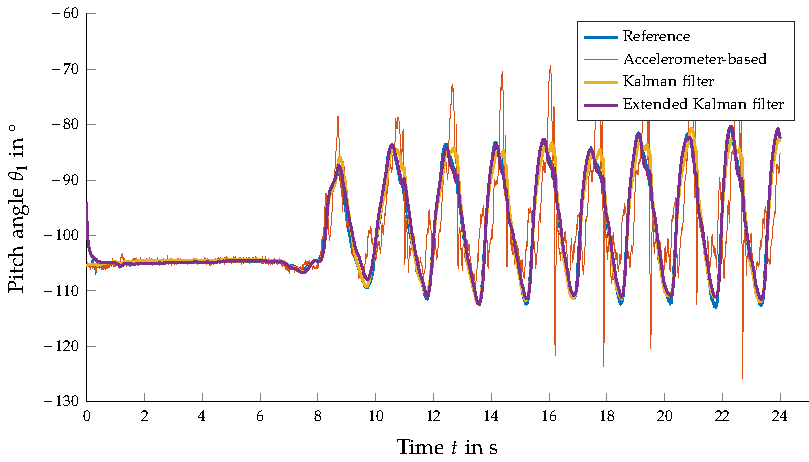
\includegraphics[width=\textwidth]{Tikz/experiment_4.tikz}
	\caption{Pitch angle of the right thigh with respect to the $x$-axis obtained by projection of the gravity vector, classical Kalman filtering, and extended Kalman filtering, in comparison to the reference. Walking speed: $\unitfrac[2]{km}{h}$.}
	\label{fig:experiment_4}
\end{figure}

\begin{figure}
	\centering
	\setlength\figureheight{6.8cm} 
	\setlength\figurewidth{\textwidth}
	\tikzsetnextfilename{experiment_5}
	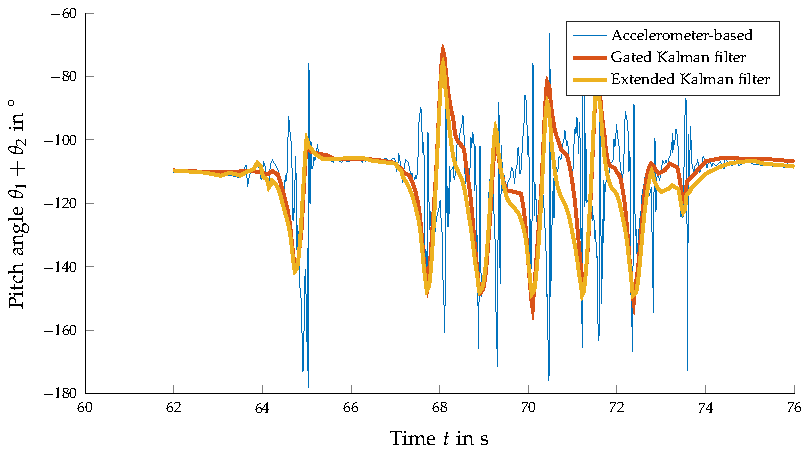
\includegraphics[width=\textwidth]{Tikz/experiment_5.tikz}
	\caption{Pitch angle of the right shank with respect to the $x$-axis obtained by projection of the gravity vector, classical Kalman filtering, and extended Kalman filtering, in comparison to the reference. Walking speed: $\unitfrac[2]{km}{h}$.}
	\label{fig:experiment_5}
\end{figure}

\begin{figure}
	\centering
	\setlength\figureheight{7cm} 
	\setlength\figurewidth{\textwidth}
	\tikzsetnextfilename{experiment_6}
	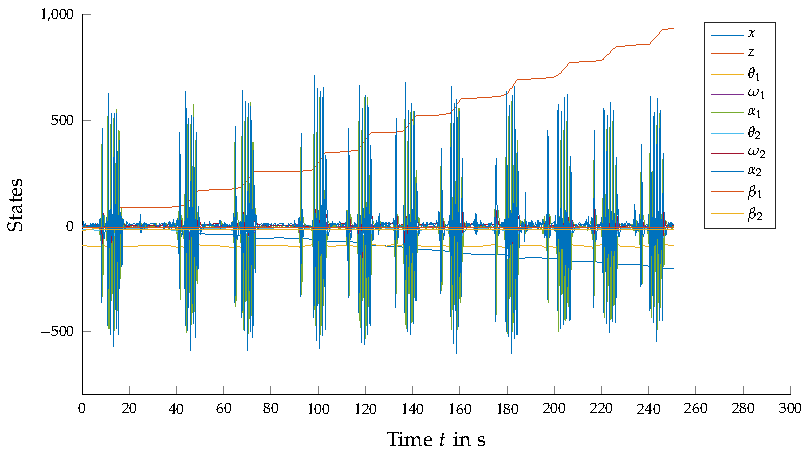
\includegraphics[width=\textwidth]{Tikz/experiment_6.tikz}
	\caption{Root-mean-square error comparison of angle estimation by projection of the gravity vector, classical Kalman filtering, and extended Kalman filtering. Walking speed: $\unitfrac[2]{km}{h}$.}
	\label{fig:experiment_6}
\end{figure}

\begin{figure}
	\centering
	\setlength\figureheight{7cm} 
	\setlength\figurewidth{\textwidth}
	\tikzsetnextfilename{experiment_7}
	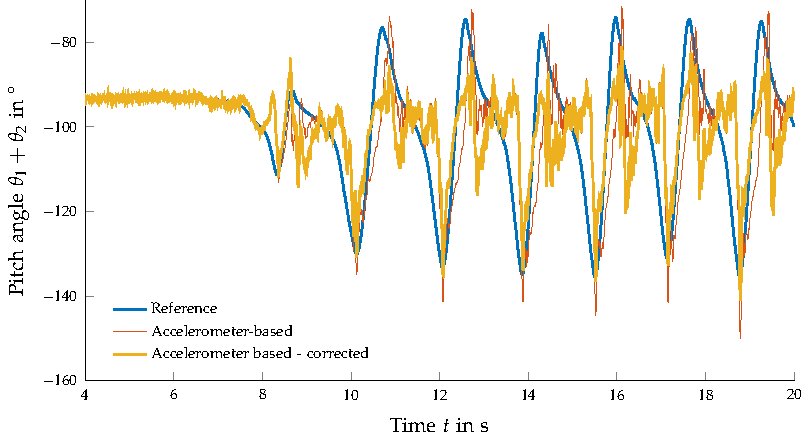
\includegraphics[width=\textwidth]{Tikz/experiment_7.tikz}
	\caption{Accelerometer-based shank angle with respect to the $x$-axis with and without correction of acceleration signal. Walking speed: $\unitfrac[2]{km}{h}$.}
	\label{fig:experiment_7}
\end{figure}

\begin{figure}
	\centering
	\setlength\figureheight{6.8cm} 
	\setlength\figurewidth{\textwidth}
	\tikzsetnextfilename{experiment_8}
	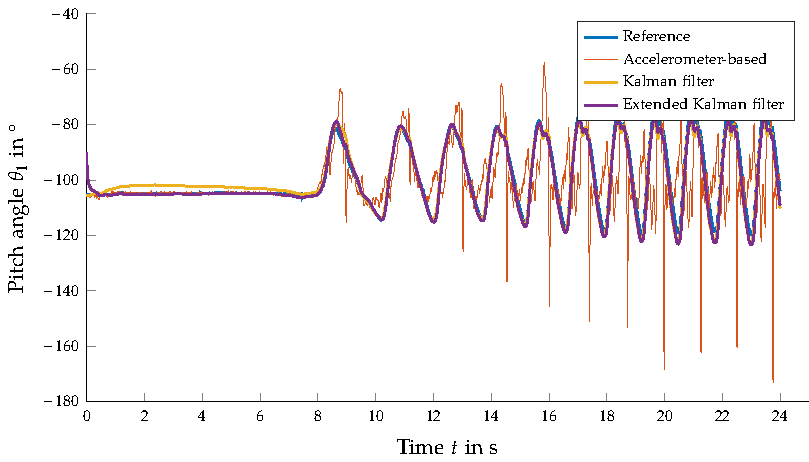
\includegraphics[width=\textwidth]{Tikz/experiment_8.tikz}
	\caption{Pitch angle of the right thigh with respect to the $x$-axis obtained by projection of the gravity vector, classical Kalman filtering, and extended Kalman filtering, in comparison to the reference. Walking speed: $\unitfrac[4]{km}{h}$.}
	\label{fig:experiment_8}
\end{figure}

\begin{figure}
	\centering
	\setlength\figureheight{6.8cm} 
	\setlength\figurewidth{\textwidth}
	\tikzsetnextfilename{experiment_9}
	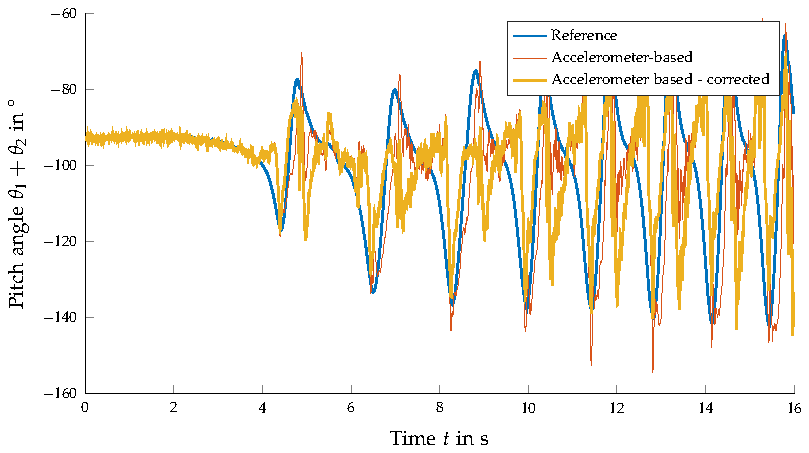
\includegraphics[width=\textwidth]{Tikz/experiment_9.tikz}
	\caption{Pitch angle of the right shank with respect to the $x$-axis obtained by projection of the gravity vector, classical Kalman filtering, and extended Kalman filtering, in comparison to the reference. Walking speed: $\unitfrac[4]{km}{h}$.}
	\label{fig:experiment_9}
\end{figure}

\begin{figure}
	\centering
	\setlength\figureheight{7cm} 
	\setlength\figurewidth{\textwidth}
	\tikzsetnextfilename{experiment_10}
	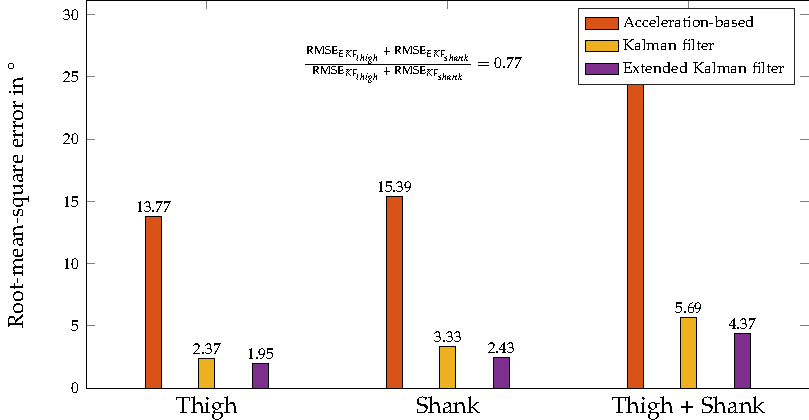
\includegraphics[width=\textwidth]{Tikz/experiment_10.tikz}
	\caption{Root-mean-square error comparison of angle estimation by projection of the gravity vector, classical Kalman filtering, and extended Kalman filtering. Walking speed: $\unitfrac[4]{km}{h}$.}
	\label{fig:experiment_10}
\end{figure}

\begin{figure}
	\centering
	\setlength\figureheight{7cm} 
	\setlength\figurewidth{\textwidth}
	\tikzsetnextfilename{experiment_11}
	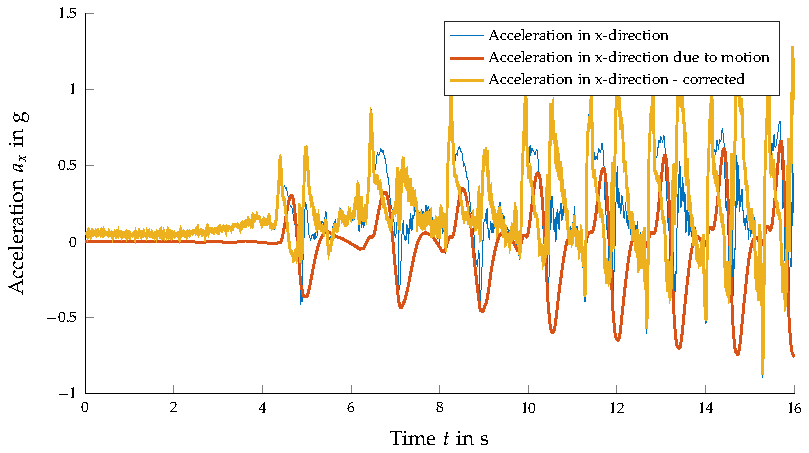
\includegraphics[width=\textwidth]{Tikz/experiment_11.tikz}
	\caption{Accelerometer-based shank angle with respect to the $x$-axis with and without correction of acceleration signal. Walking speed: $\unitfrac[4]{km}{h}$.}
	\label{fig:experiment_11}
\end{figure}

\begin{figure}
	\centering
	\setlength\figureheight{6.8cm} 
	\setlength\figurewidth{\textwidth}
	\tikzsetnextfilename{experiment_12}
	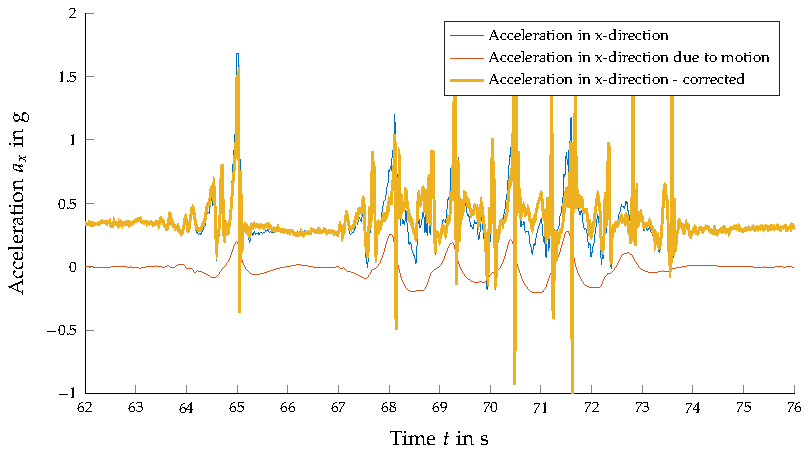
\includegraphics[width=\textwidth]{Tikz/experiment_12.tikz}
	\caption{Pitch angle of the right thigh with respect to the $x$-axis obtained by projection of the gravity vector, classical Kalman filtering, and extended Kalman filtering, in comparison to the reference. Walking speed: $\unitfrac[6]{km}{h}$.}
	\label{fig:experiment_12}
\end{figure}

\begin{figure}
	\centering
	\setlength\figureheight{6.8cm} 
	\setlength\figurewidth{\textwidth}
	\tikzsetnextfilename{experiment_13}
	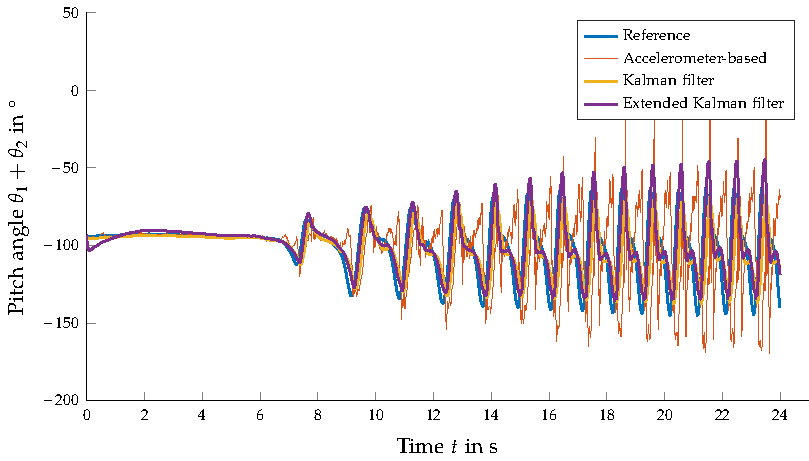
\includegraphics[width=\textwidth]{Tikz/experiment_13.tikz}
	\caption{Pitch angle of the right shank with respect to the $x$-axis obtained by projection of the gravity vector, classical Kalman filtering, and extended Kalman filtering, in comparison to the reference. Walking speed: $\unitfrac[6]{km}{h}$.}
	\label{fig:experiment_13}
\end{figure}

\begin{figure}
	\centering
	\setlength\figureheight{7cm} 
	\setlength\figurewidth{\textwidth}
	\tikzsetnextfilename{experiment_14}
	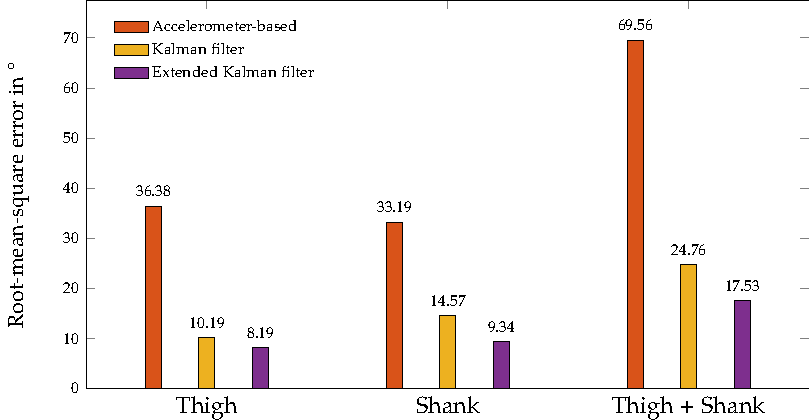
\includegraphics[width=\textwidth]{Tikz/experiment_14.tikz}
	\caption{Root-mean-square error comparison of angle estimation by projection of the gravity vector, classical Kalman filtering, and extended Kalman filtering. Walking speed: $\unitfrac[6]{km}{h}$.}
	\label{fig:experiment_14}
\end{figure}

\begin{figure}
	\centering
	\setlength\figureheight{7cm} 
	\setlength\figurewidth{\textwidth}
	\tikzsetnextfilename{experiment_15}
	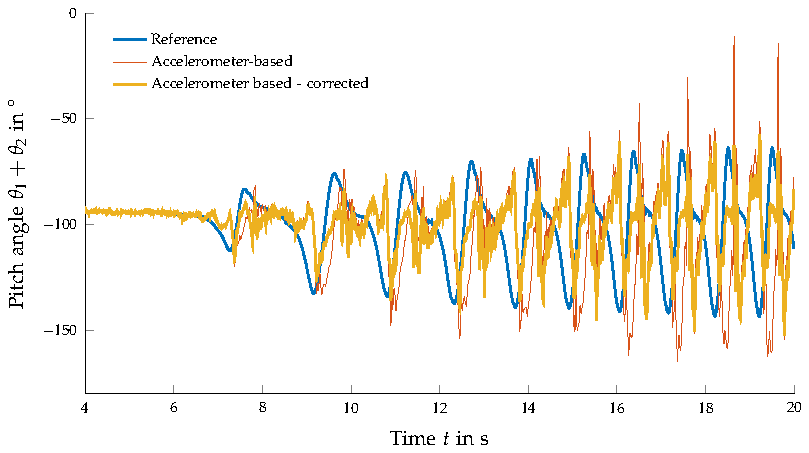
\includegraphics[width=\textwidth]{Tikz/experiment_15.tikz}
	\caption{Accelerometer-based shank angle with respect to the $x$-axis with and without correction of acceleration signal. Walking speed: $\unitfrac[6]{km}{h}$.}
	\label{fig:experiment_15}
\end{figure}

\section{Discussion}

After the presentation of the results, we now proceed to analysing them in detail. The RMSEs of the motion-corrected accelerometer-basedased angle estimates while walking at $\unitfrac[2]{km}{h}$ and $\unitfrac[4]{km}{h}$ were only slightly different from the raw accelerometer-basedased angle estimates. This could be explained by the simple kinematic model of the leg. Even though it considers the motion of the leg in $x$ and $z$-direction with respect to the origin of the world coordinate frame, that is the hip joint, it does not consider motion of the entire system itself. However, while walking, the human body rotates about the hip joint, which causes motion of the respective opposite hip joint. Additionally, the tension of the calf muscles and the resulting stretching of the foot moves the entire body upwards, including the hip joint. That means that the origin of the world coordinate frame of the kinematic model moves, contrary to the assumption made in the model. This movement causes not only an additional acceleration component in the sensor signal while moving the leg in the air, but also a quite severe impact on the acceleration signal when touching the ground with the foot. Another fact that is not considered in the simple model, is motion beyond the $xz$-plane. Finally, the lengths of the links, i.\,e. the sensor position on the thigh and shank was not exactly known. As the trend of the relative RMSEs of the accelerometer-basedased angle estimates shows, the motion correction works better for faster motions. 

 Even though the acceleration correction does not benefit the RMSE of the accelerometer-basedased angle estimate for walking speeds of $\unitfrac[2]{km}{h}$ and $\unitfrac[4]{km}{h}$, the improvement of the filter output is significant for all three walking speeds. This improvement could be caused by a better filter tuning. The parameters found in an optimisation process, are not necessarily optimal. Due to the fact that the optimiser does not consider all possible combinations of the parameters, but instead finds local minima of the error function, the parameters may still be somewhat less than optimal and are strongly dependent on the initial guess. As one can see in Figures \ref{fig:experiment_7}, \ref{fig:experiment_11}, and \ref{fig:experiment_15}, the motion-based acceleration correction improves the angle estimate in some intervals, but even worsens it in others. The Kalman filter compensates those deviations trusting on the state-space model. The newly implemented filter algorithm is based on a more complete state-space model, for instance it combines information about both thigh and shank in the same state-space model, which could be one reason why it delivers a more accurate estimate.
